\section{Test cases}
\label{section:cases}

\begin{itemize}
	\item Two test cases were implemented to drive the adapter development
	\item The OpenFAST simulation of a single NREL 5MW turbine \cite{Jonkman:2009} should be coupled
	\item Coupling to dummy fluid solver to test the data exchange
	\item Coupling to OpenFOAM to test the mapping with a CFD tool
	\item Both cases are part of the repository on GitHub\footnote{\url{https://github.com/LeonardWilleke/openfast-adapter/tree/main/cases}}\\
\end{itemize}

Case dummy-turbine
\begin{itemize}
	\item Explain the setup
	\begin{itemize}
		\item Couple OpenFAST to a dummy fluid solver
		\item OpenFAST computes a NREL 5MW turbine with a fixed rotor to avoid problems due to the moving mesh
		\item Fluid solver is implemented as dummy: No CFD calculation takes place
		\item The dummy creates a mesh on which data from OpenFAST is read and writes back constant values
		\item Allows to explore the mapping and data exchange
		\item Can be used for regression tests in the future
	\end{itemize}
	\item Explain the mesh use of OpenFAST
	\begin{itemize}
		\item OpenFAST has two internal meshes of the turbine surface with different vertices
		\item Force mesh: Used to store and compute the surface force
		\item Velocity mesh: Used to store and compute the flow velocity
		\item Possibility to let OpenFAST map between the two meshes
		\item Both meshes can be accessed via the C++ API
		\item We want to use preCICE for the mapping
		\item A similar coupling setup is employed by \cite{Taschner:2022} who also uses both meshes
		\item Maybe add a visualization of the coupling scheme to clarify the mesh use\\
	\end{itemize}
\end{itemize}

Case cfd-turbine
\begin{itemize}
	\item Explain the setup
	\begin{itemize}
		\item Couple OpenFAST to OpenFOAM
		\item The coupling scheme and mesh use is identical to the dummy
		\item Now we are dealing with a different mesh on the fluid solver
		\item Main obstacle: The OpenFOAM adapter is not designed to implement a coupling with a solver using the actuator line method. How to map between the line mesh in OpenFAST (Figure )\ref{fig:mesh:fast} and the volume mesh in OpenFOAM (Figure \ref{fig:mesh:foam})?
	\end{itemize}
	\item Explain how the current setup works
	\begin{itemize}
		\item Define a cellSet inside the OpenFOAM domain (Figure \ref{fig:mesh:foam}) to which OpenFAST is coupled
		\item Write the rotor and tower data to this subdomain
		\item Read velocity data from this subdomain
		\item The mapping from line to volume and back is done by preCICE, but probably wrong
	\end{itemize}
	\item How should the turbine be represented in OpenFOAM?
	\begin{itemize}
		\item Volume mesh / cellSet
		\item Surface mesh / patch
		\item ALM implementation (eg with turbinesFoam)\\
	\end{itemize}
\end{itemize}

\begin{figure*}[h]
	\centering
	\begin{subfigure}{0.7\textwidth}
		\centering
		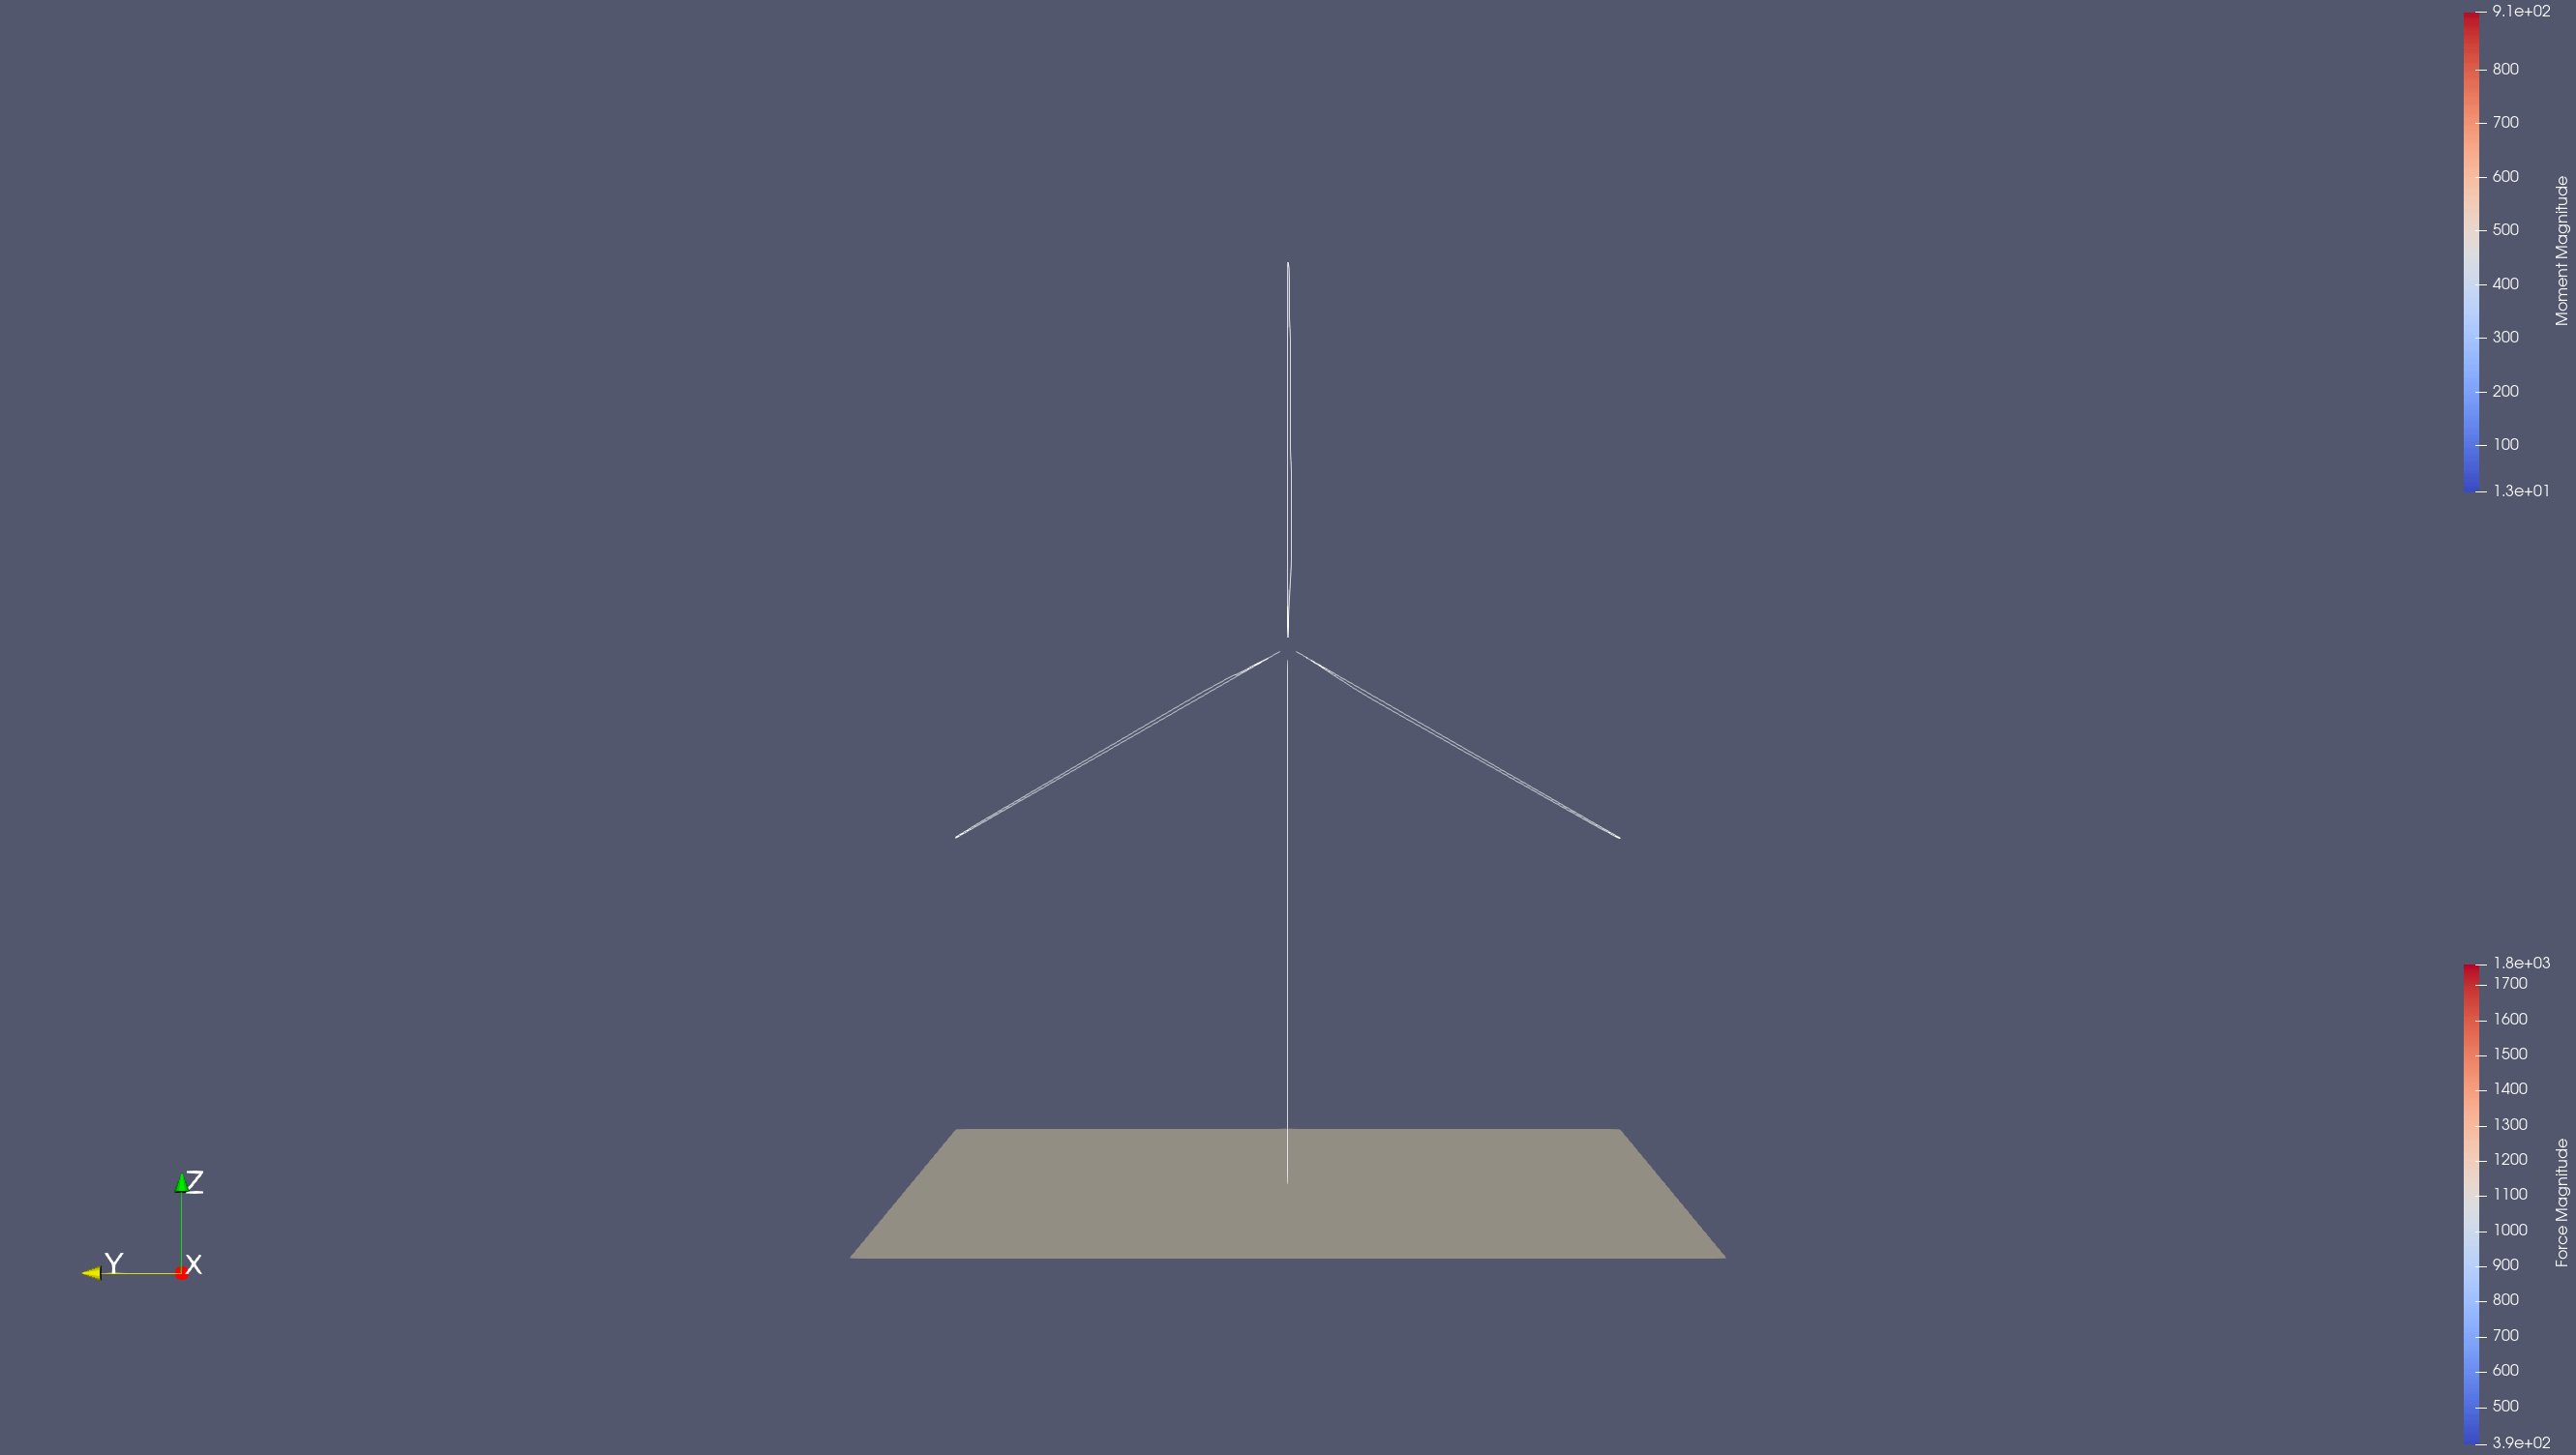
\includegraphics[width=\linewidth]{images/openfast-turbine-mesh.png}
		\caption{Line representation of the turbine in OpenFAST}
		\label{fig:mesh:fast}
	\end{subfigure}
	\vspace{2pt}
	\begin{subfigure}{0.7\textwidth}
		\centering
		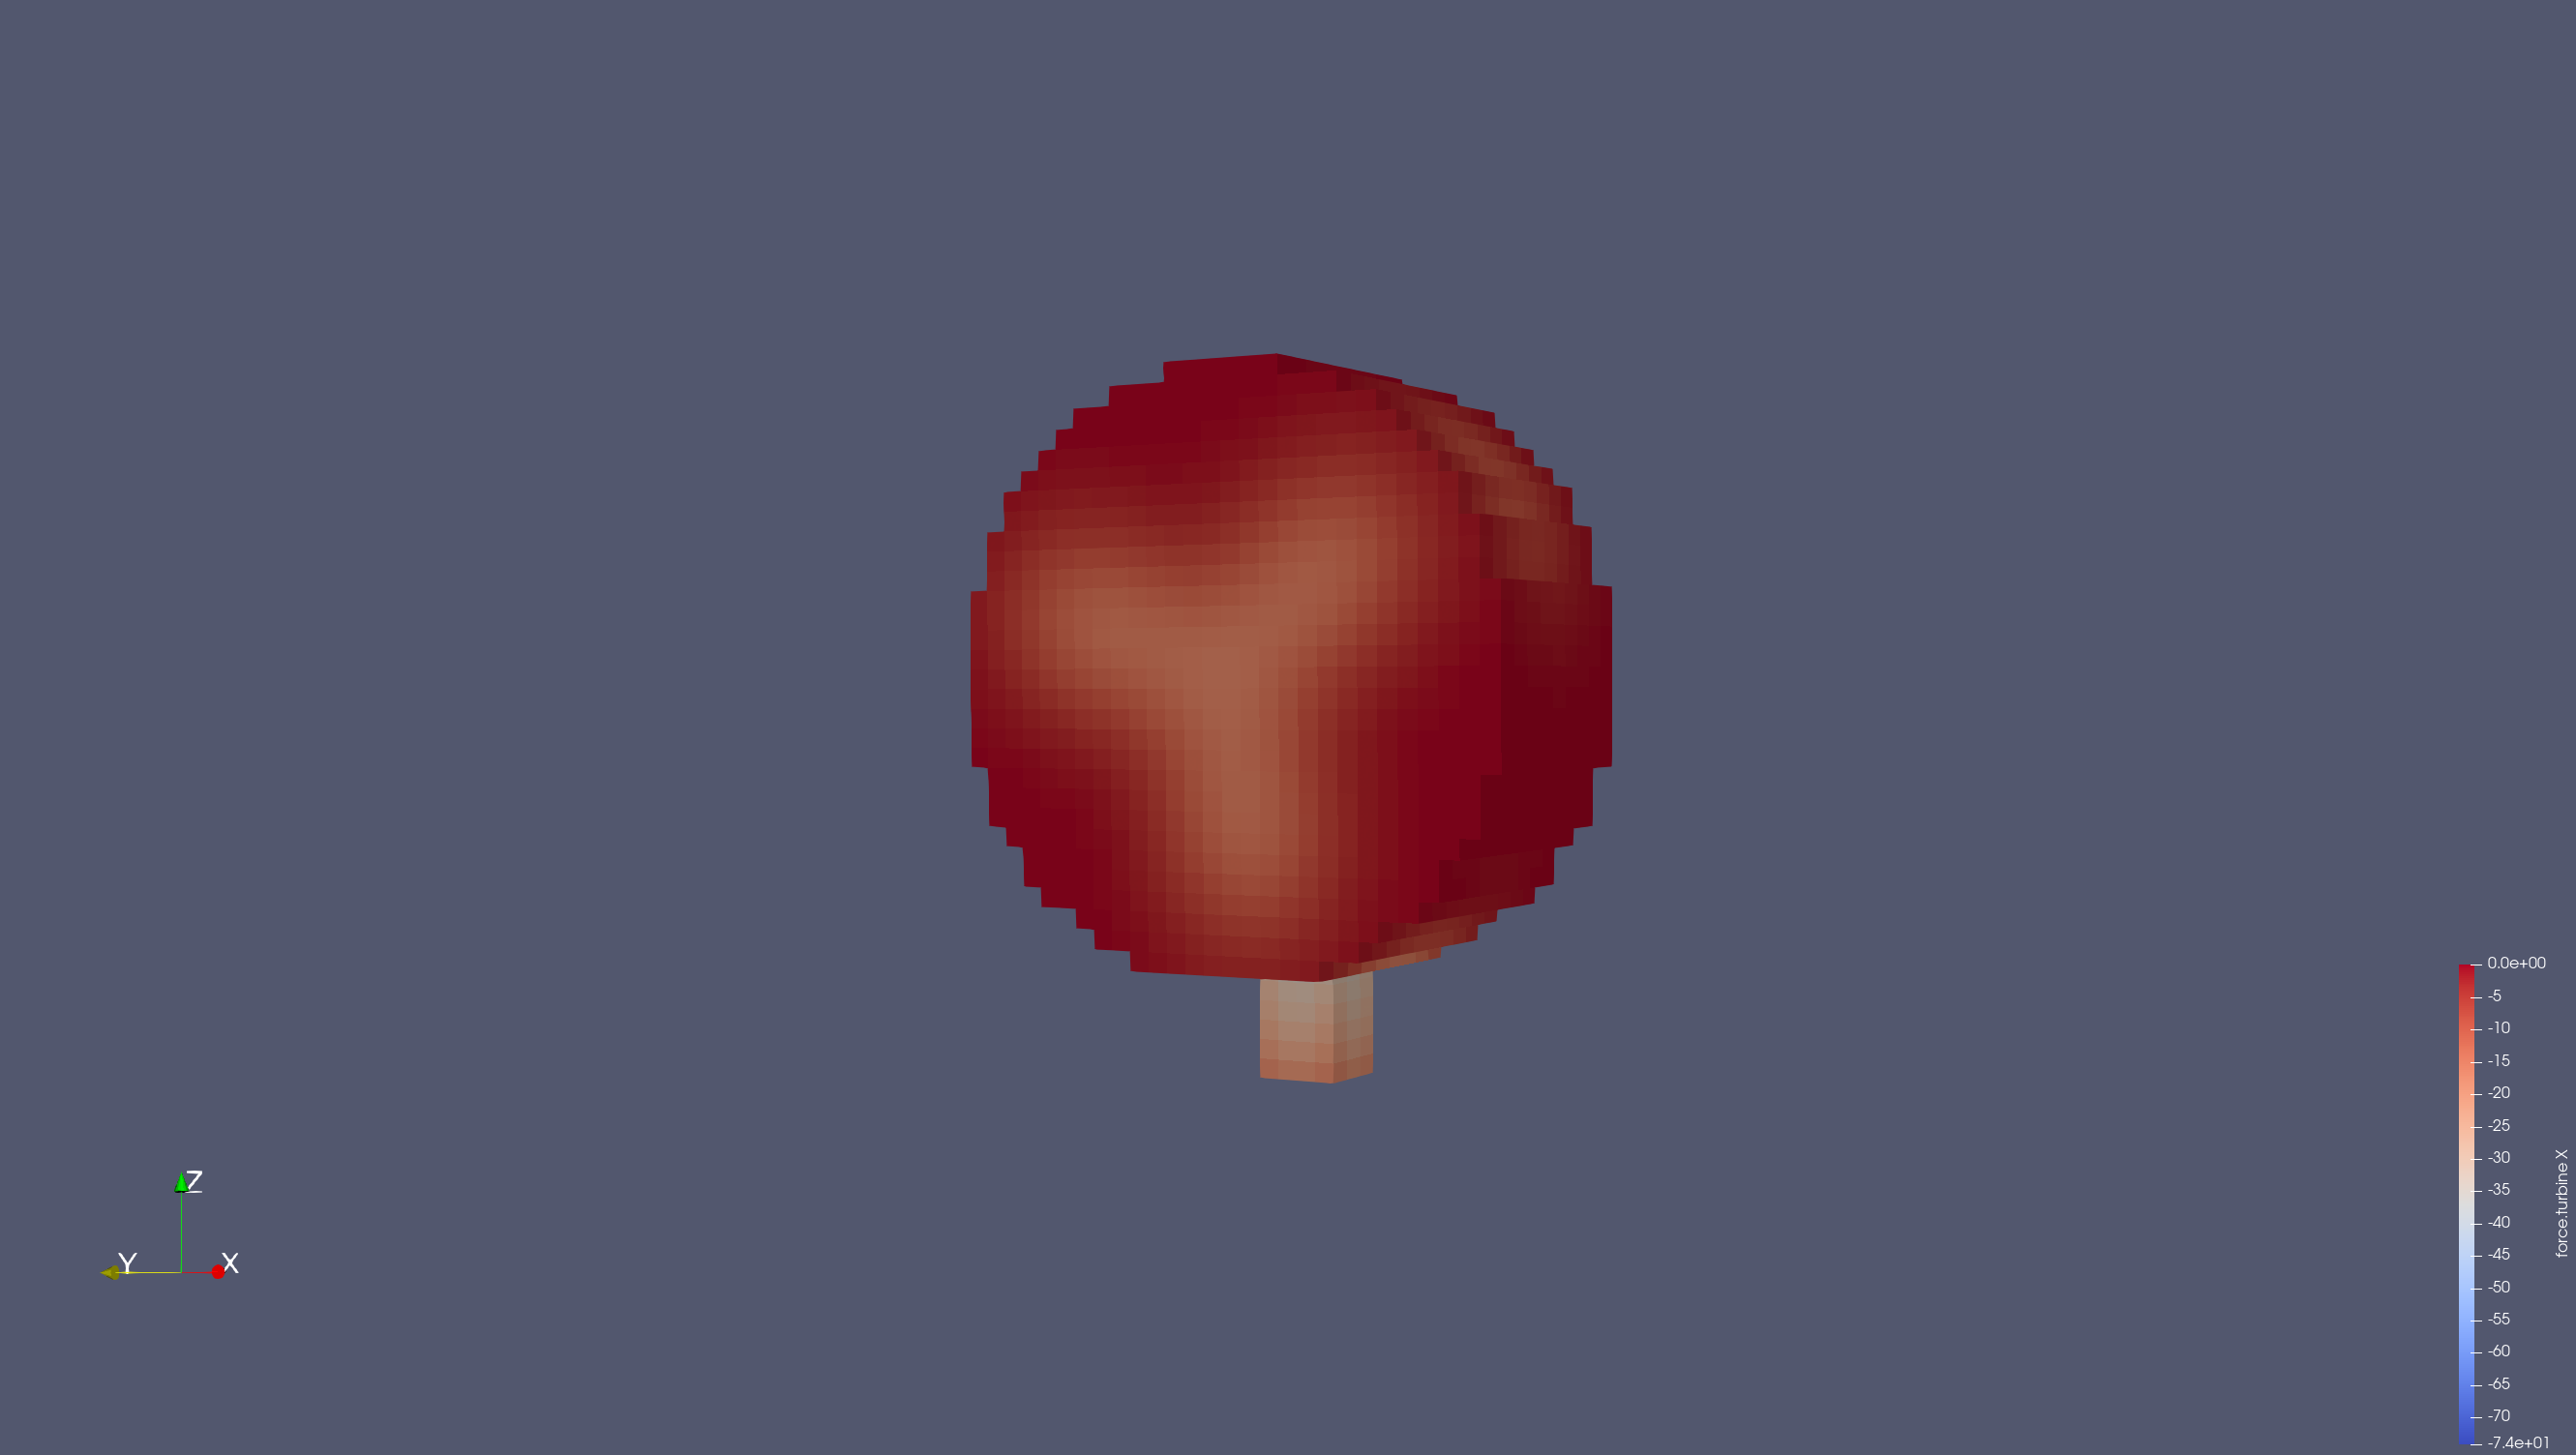
\includegraphics[width=\linewidth]{images/openfoam-turbine-mesh.png}
		\caption{Volume representation of the flow field immediately around the turbine in OpenFOAM}
		\label{fig:mesh:foam}
	\end{subfigure}
	\caption{Mesh differences between OpenFAST and the CFD solver OpenFOAM. OpenFAST uses the Actuator Line Model to represent blades and towers in the flow field, while OpenFOAM calculates the whole flow field.}
	\label{fig:mesh}
\end{figure*}

